% VDE Template for EUSAR Papers
% Provided by Barbara Lang und Siegmar Lampe
% University of Bremen, January 2002
% English version by Jens Fischer
% German Aerospace Center (DLR), December 2005
% Additional modifications by Matthias Wei{\ss}
% FGAN, January 2009

%-----------------------------------------------------------------------------
% Type of publication
\documentclass[a4paper,10pt]{article}
%-----------------------------------------------------------------------------
% Other packets: Most packets may be downloaded from www.dante.de and
% "tcilatex.tex" can be found at (December 2005):
% http://www.mackichan.com/techtalk/v30/UsingFloat.htm
% Not all packets are necessarily needed:
\usepackage[T1]{fontenc}
\usepackage[latin1]{inputenc}
%\usepackage{ngerman} % in german language if required
\usepackage[nooneline,bf]{caption} % Figure descriptions from left margin
\usepackage{times}
\usepackage{multicol}
\usepackage{amsmath}
\usepackage{amssymb}
\usepackage[dvips]{graphicx}
\usepackage{epsfig}
\usepackage{hyperref}
\usepackage[justification=centering]{caption}
\input{tcilatex}
%-----------------------------------------------------------------------------
% Page Setup
\textheight24cm \textwidth17cm \columnsep6mm
\oddsidemargin-5mm                 % depending on print drivers!
\evensidemargin-5mm                % required margin size: 2cm
\headheight0cm \headsep0cm \topmargin0cm \parindent0cm
\pagestyle{empty}                  % delete footer and header
%----------------------------------------------------------------------------
% Environment definitions
\newenvironment*{mytitle}{\begin{LARGE}\bf}{\end{LARGE}\\}%
\newenvironment*{mysubtitle}{\bf}{\\[1.5ex]}%
\newenvironment*{myabstract}{\begin{Large}\bf}{\end{Large}\\[2.5ex]}%
%-----------------------------------------------------------------------------
% Using Pictures and tables:
% - Instead "table" write "tablehere" without parameters
% - Instead "figure" write "figurehere " without parameters
% - Please insert a blank line before and after \begin{figuerhere} ... \end{figurehere}
%
% CAUTION:   The first reference to a figure/table in the text should be formatted fat.
%
\makeatletter
\newenvironment{tablehere}{\def\@captype{table}\vspace{2ex}}{\vspace{1ex}}
\newenvironment{figurehere}{\def\@captype{figure}\vspace{2ex}}{\vspace{1ex}}
\makeatother



%%%%%%%%%%%%%%%%%%%%%%%%%%%%%%%%%%%%%%%%%%%%%%%%%%%%%%%%%%%%%%%%%%%%%%%%%%%%%%
\begin{document}

% Please use capital letters in the beginning of important words as for example
\begin{mytitle}Pedometer for STM32F4\end{mytitle}
\begin{mysubtitle}Use the MEMS accelerometer to count number of steps\end{mysubtitle}
%
% Please do not insert a line here
%
\\
De Donatis Emanuele\\
Matr. 817667, (emanuele.dedonatis@mail.polimi.it)\\
\hspace{10ex}
Pistone Bruno\\
Matr. 818949, (bruno.pistone@mail.polimi.it)\\
\begin{flushright}
\emph{Report for the master course of Embedded Systems}\\
\end{flushright}

July, 18 2014\\
\hspace{10ex}

\begin{myabstract} Abstract \end{myabstract}
This project is part of a collaborative project whose purpose is to develop a simple 
yet realistic training support system. The goal of this project is to develop a pedometer 
using the MEMS motion sensor on the STM32F4DISCOVERY board. The device provides
the user with statistics about its training activity.

\vspace{4ex}	% Please do not remove or reduce this space here.
\begin{multicols}{2}

%%%%%%%%%%%%%%%%%%%%%%%%%%%%%%%%%%%%%%%%%%%%%%%%%%%%%%%%%%%%%%%%%%%%%%%%%%%%%
\section{Introduction}
The Real-Time Operating System course of the Polytechnic of Milan proposed a collaborative project whose aim is to develop a Personal Trainer device
based on the economical development board STM32F4DISCOVERY and the 
Miosix embedded OS. 


\begin{tablehere}
\centering
\begin{tabular}{|c|l|} \hline
{\bf Module Name} & {\bf Device}\\ \hline
Pedometer & MEMS \\
User Interface & UART, Flash\\
Audio Feedback & CS43L22 (DAC) \\
Voice Commands & NONE (PCM Samples) \\
PCM Encoding & MP45DT02 MEMS Mic\\
Social Wireless & NRF24L01 2.4GHz TxRx\\
Context Awareness & ADC \\ \hline
\end {tabular}
\caption{Group modules} 
\end{tablehere} 


The final goal is to join each module in order to build a working system.

%-----------------------------------------------------------------------------
\subsection{STM32F4DISCOVERY board}
% Please avoid separations in titles
% and separate text manually

The STM32F4DISCOVERY is an evaluation board by STMicroelectronics, based on the ARM Cortex-M4F core.

{\small
\begin{itemize}
\item STM32F407VGT6 microcontroller featuring 32-bit ARM Cortex-M4F core, 1 MB Flash, 192 KB RAM in an LQFP100 package
\item LIS302DL or LIS3DSH ST MEMS 3-axis accelerometer
\item MP45DT02, ST MEMS audio sensor, omni-directional digital microphone
\item CS43L22, audio DAC with integrated class D speaker driver
\item USB OTG FS with micro-AB connector
\end{itemize}
}

\begin{figurehere}
 \centering
 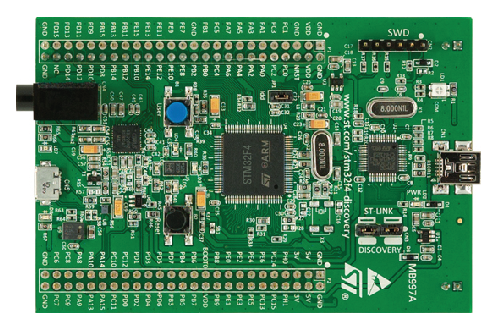
\includegraphics[width=8cm, height=5cm]{./eps/STM32F4.eps}
 \caption{STM32F4DISCOVERY board}
 \label{fig:STM32F4}
\end{figurehere}

%-----------------------------------------------------------------------------
\subsection{MIOSIX embedded OS}
% Please avoid separations in titles
% and separate text manually

Miosix is an OS kernel designed to run on 32bit microcontrollers, in active development since 2008.
It supports both a single process, multiple threads application model where applications are statically linked with the kernel, and an experimental multiprocess environment with memory protection that allows loading applications at runtime. 
The kernel is royalty-free and licensed under the GPL license with an exception that allows it to be linked with propietary application code. \cite{miosix}

%-----------------------------------------------------------------------------
\subsection{MEMS Motion Sensor}
% Please avoid separations in titles
% and separate text manually

The STM32F4DISCOVERY includes the LIS302DL ST MEMS motion sensor.
It is an ultra compact low-power three-axis linear accelerometer. It includes
a sensing element and an IC interface able to provide the measured acceleration
to the external world through I2C/SPI serial interface.

The STM32F4 controls this motion sensor through the SPI interface (see {\bf Figure
\ref{fig:LIS302DL}}). 

\begin{figurehere}
 \centering
 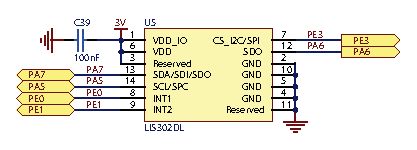
\includegraphics[width=8cm, height=3cm]{./eps/LIS302DL.eps}
 \caption{LIS302DL Motion Sensor}
 \label{fig:LIS302DL}
\end{figurehere}

%%%%%%%%%%%%%%%%%%%%%%%%%%%%%%%%%%%%%%%%%%%%%%%%%%%%%%%%%%%%%%%%%%%%%%%%%%%%%
\section{Pedometer Algorithm}

To develop the pedometer algorithm we relied on the Neil Zhao's model .\cite{NeilZhao}


%-----------------------------------------------------------------------------
\subsection{Digital Filter}

A digital filter is needed to smooth the signals. Four registers and a summing unit can be used  (see {\bf Figure
\ref{fig:DigitalFilter}}).  More registers could be used to make the acceleration data smoother, but the response time would be slower.

\begin{figurehere}
 \centering
 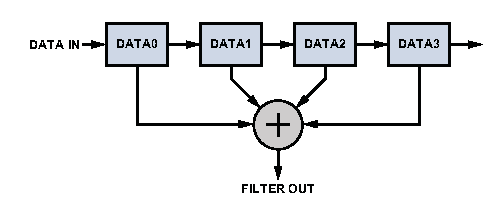
\includegraphics[width=7cm, height=3cm]{./eps/DigitalFilter.eps}
 \caption{Digital filter}
 \label{fig:DigitalFilter}
\end{figurehere}

%-----------------------------------------------------------------------------
\subsection{Dynamic Threshold and Dynamic Precision}

The system updates the maximum and minimum values of the 3-axis acceleration every 50 samples. The average value, (Max + Min)/2, is called the dynamic threshold level. 

\begin{figurehere}
 \centering
 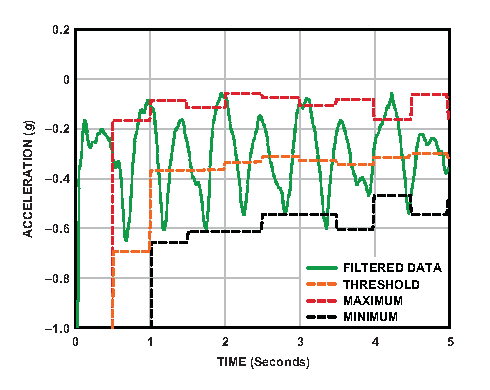
\includegraphics[width=8cm, height=5cm]{./eps/Threshold.eps}
 \caption{Acceleration curves}
 \label{fig:Threshold}
\end{figurehere}

For each axis two registers, sample\textunderscore new and sample\textunderscore old, are used to pick out new sample result. When a new data sample comes, sample\textunderscore new is shifted to the sample\textunderscore old register unconditionally. However the new sample result will be shifted into the sample\textunderscore new register only if the changes in acceleration are greater than a predefined precision; otherwise the sample\textunderscore new register will remain unchanged. The shift register group can thus remove the high-frequency noise and make the decision more precise.

\begin{figurehere}
 \centering
 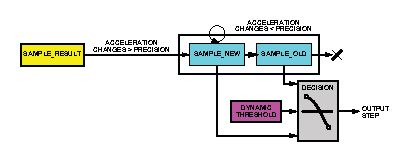
\includegraphics[width=8cm, height=3cm]{./eps/RegistersDiagram.eps}
 \caption{Dynamic threshold and dynamic precision}
 \label{fig:RegistersDiagram}
\end{figurehere}

%-----------------------------------------------------------------------------
\subsection{Step}

A step is defined as happening if there is a negative slope of the acceleration plot (sample\textunderscore new < sample\textunderscore old) when the vertical acceleration curve crosses below the dynamic threshold.

%-----------------------------------------------------------------------------
\subsection{Peak Detection}

The step counter calculates the steps from the x-axis, y-axis, or z-axis, depending on which axis has the maximum absolute value of threshold, since the gravitational force acts on it.

%-----------------------------------------------------------------------------
\subsection{Time Window}

Time window is used to discard the invalid vibrations. We assume that people can run as rapidly as five steps per second and walk as slowly as one step every two seconds. Thus, the interval between two valid steps is defined as being in the time window [0.2 s to 2.0 s]; all steps with intervals outside the time window should be discarded.

%%%%%%%%%%%%%%%%%%%%%%%%%%%%%%%%%%%%%%%%%%%%%%%%%%%%%%%%%%%%%%%%%%%%%%%%%%%%%
\section{Statistics}

%-----------------------------------------------------------------------------
\subsection{Training mode}

It is possible to recognize the training mode based on the step's frequency: the running frequency is between 2 and 5 steps per second and the walking frequency is between 0.5 and 2 steps per second. 

\begin{tablehere}
\centering
\begin{tabular}{|c|c|c|} \hline
{\bf Minimum} & {\bf Mode} & {\bf Maximum}\\ \hline
200ms & RUNNING & 500ms \\
500ms & WALKING & 2000ms \\
2000ms & STEADY & $\infty$ \\  \hline
\end{tabular}
\caption{Interval time between two steps}
\end{tablehere}



%-----------------------------------------------------------------------------
\subsection{Distance}

The distance depends on the length of a step. Experimentally we can approximate this length as: \\

\centerline{$walking \_ length = 1/6 * height$}
\centerline{$running \_ length = 1/3 * height$}

%-----------------------------------------------------------------------------
\subsection{Speed}
Knowing the distance and the time between two steps we can calculate the approximate speed: \\

\centerline{$speed = distance / time$}

%-----------------------------------------------------------------------------
\subsection{Calories}
There is no accurate means for calculating the rate of expending calories. 
Some factors that determine it include body weight, intensity of workout, conditioning level, and metabolism.
We can estimate it using a conventional approximation: \\

\centerline{$calories [kCal] = 0.9 * distance [km] * weight [kg]$}

%%%%%%%%%%%%%%%%%%%%%%%%%%%%%%%%%%%%%%%%%%%%%%%%%%%%%%%%%%%%%%%%%%%%%%%%%%%%%
\section{User Interface}
%-----------------------------------------------------------------------------
\subsection{LCD HD44780}
We used an LCD HD44780 20x4 display to allow the user to view their own statistics. Miosix provides a C++ library to easy use the LCD.

\begin{figurehere}
 \centering
 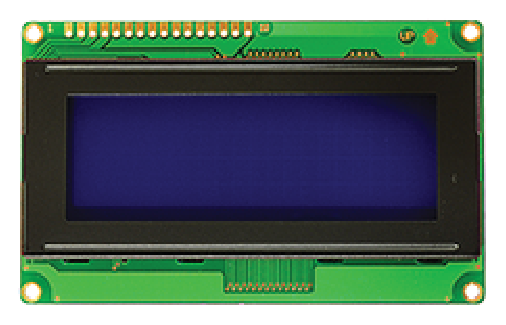
\includegraphics[width=6cm, height=3cm]{./eps/hd44780.eps}
 \caption{LCD HD44780 20x4}
 \label{fig:hd44780}
\end{figurehere}

The user can view the steps, the training mode, the instantaneous speed, the distance and the burned calories.

\begin{tablehere}
\centering
\scalebox{0.6}{
\begin{tabular}{|c|c|c|c|c|c|c|c|c|c|c|c|c|c|c|c|c|c|c|c|} \hline
S&T&E&P&S&:&&*&*&*&*& & & & & & & & & \\ \hline
M&O&D&E&:& &*&*&*&*&*&*& & & & & & & & \\ \hline
S&P&E&E&D&:& &*&*&.&*& &k&m&/&h& & & & \\ \hline
K&M&:& &*&*&.&*&*& &K&C&A&L&:& &*&*&*&*\\ \hline
\end{tabular}
}
\caption{GUI tamplate}
 \label{tab:GUI}
\end{tablehere}

%-----------------------------------------------------------------------------
\subsection{User buttons}
Some stats, like distance, speed and burned calories, required user's weight and height. 
On startup the system asks for this information and through three buttons the user can increase / decrease / confirm its weight and height.

%%%%%%%%%%%%%%%%%%%%%%%%%%%%%%%%%%%%%%%%%%%%%%%%%%%%%%%%%%%%%%%%%%%%%%%%%%%%%
\section{Social Wireless}
We collaborate with the group 61 to implement the wireless module. \cite{group61}

The goal is to exchange data with nearby devices using a NRF24L01 2.4GHz RF Transceiver.

The system sends and receives the number of steps in order to compare own stats with friends' stats.

%%%%%%%%%%%%%%%%%%%%%%%%%%%%%%%%%%%%%%%%%%%%%%%%%%%%%%%%%%%%%%%%%%%%%%%%%%%%%
\section{Audio Feedback}

We collaborate with the group 31 to implement the audio module. \cite{group31}

The goal is to notify the user about his number of steps and the result of steps' comparison with his friends.


%%%%%%%%%%%%%%%%%%%%%%%%%%%%%%%%%%%%%%%%%%%%%%%%%%%%%%%%%%%%%%%%%%%%%%%%%%%%%
\section{Conclusion}

This is the final prototype. On the left there is a potentiometer to adjust the contrast of the LCD. On the top there are the three user buttons and the NRF24L01 transceiver. On the right there is the audio jack
connected to a mini-speaker. We used a portable battery charger for smartphone to power the device via USB.

\begin{figurehere}
 \centering
 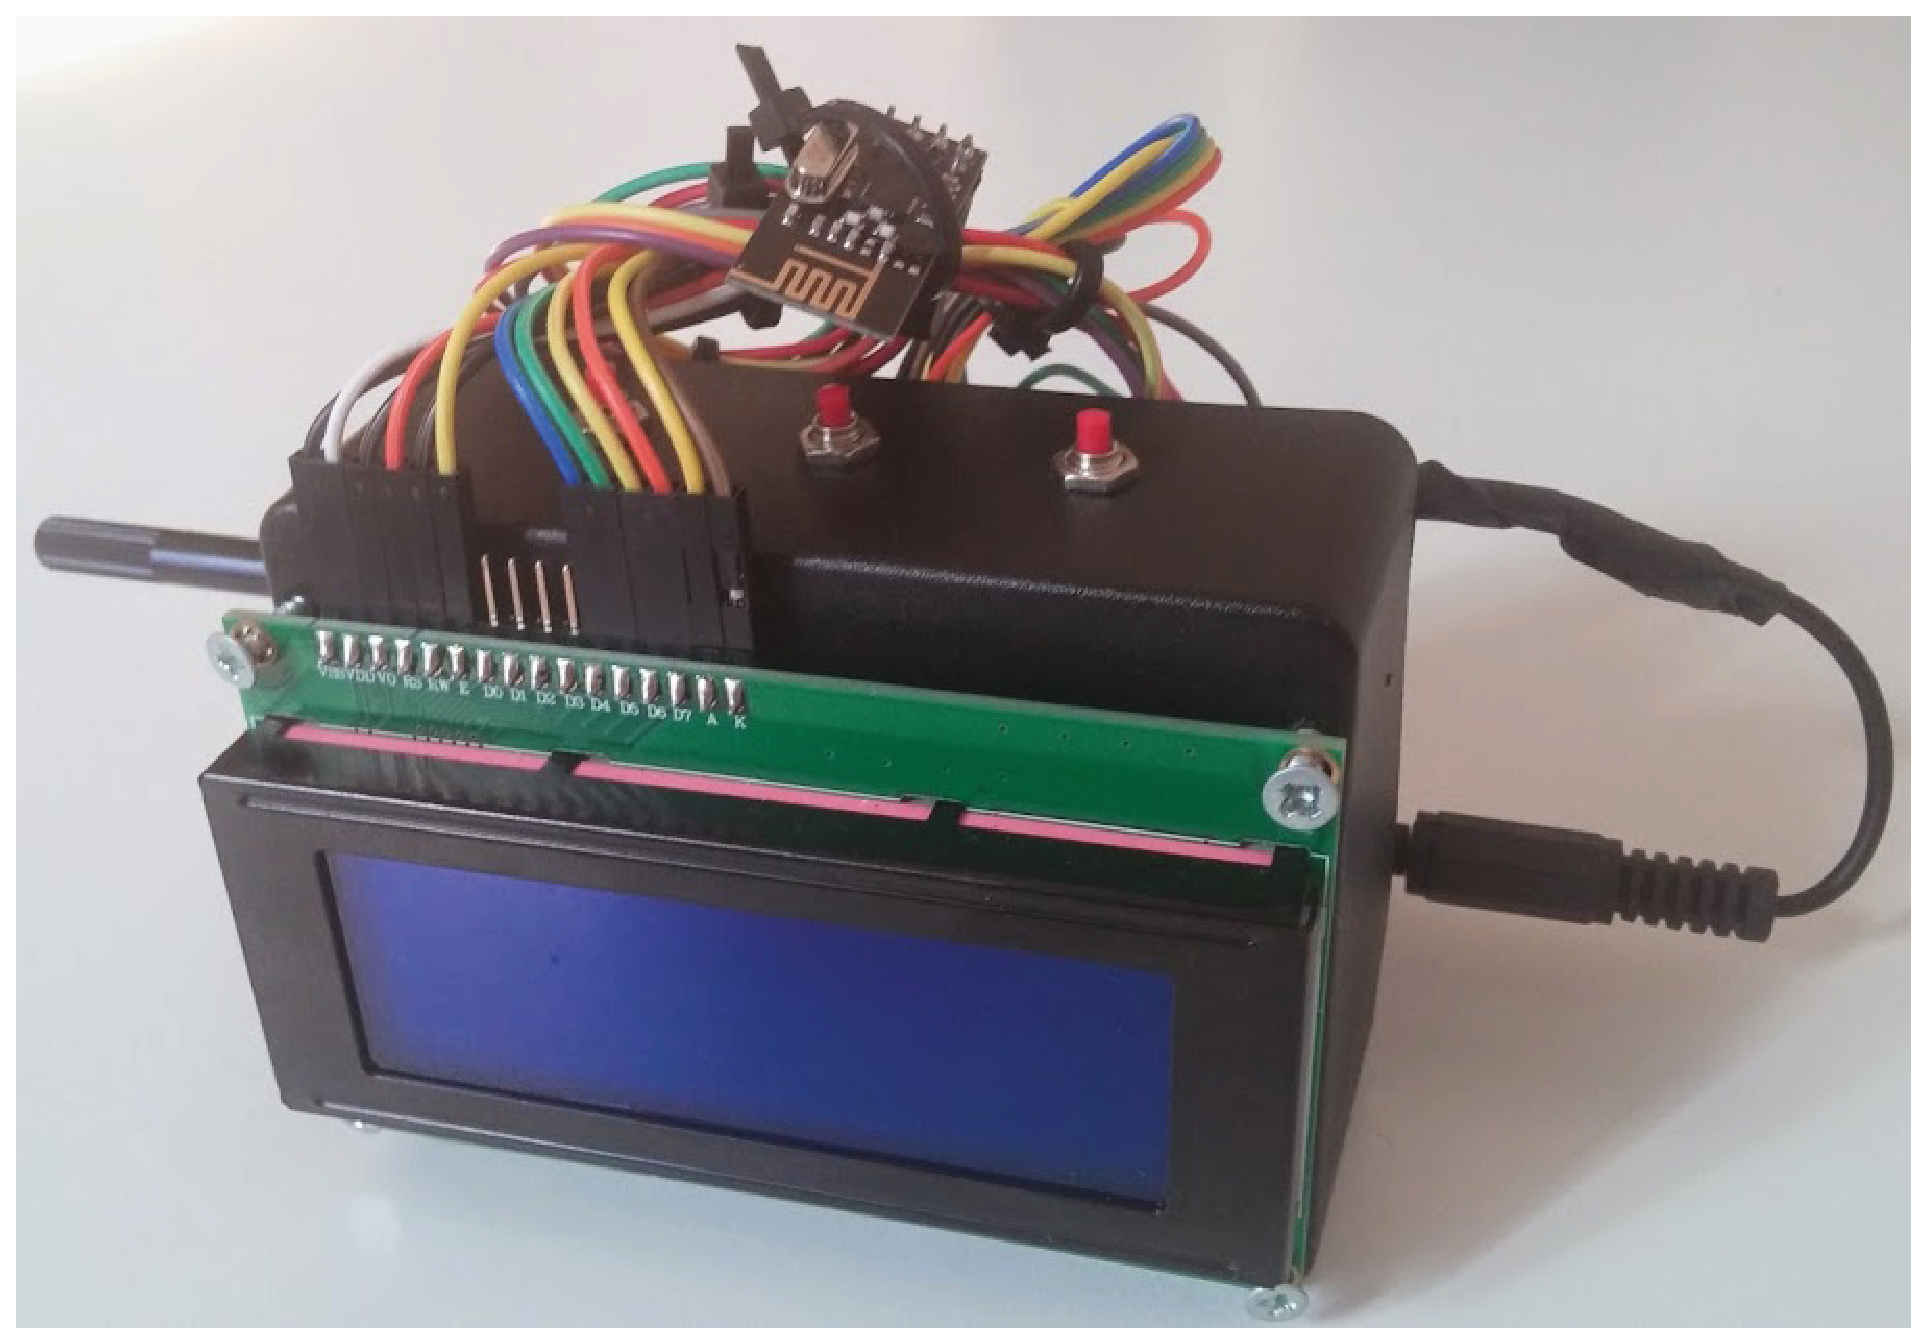
\includegraphics[width=8cm, height=5cm]{./eps/proto.eps}
 \label{fig:prototype}
\end{figurehere}

%-----------------------------------------------------------------------------
% We suggest the use of JabRef for editing your bibliography file (Report.bib)
\bibliographystyle{plain}
\bibliography{Report}

\end{multicols}
\end{document}
